\chapter{Theoretical and Technical Background}

\section{Correlation Structure}
\label{ap:Correlation}
In the book Gaussian Markov Random Fields~\cite{rue2005gaussian}, Rue and Held demonstrate that a strong correlation between the hyper-parameter $\mu$ and the latent field $\bm{x}$ can significantly slow down convergence particularly when using Gibbs samplers.  
They consider the hierarchical model

\begin{subequations}
	\begin{align}
		\mu &\sim \mathcal{N}(0, 1) \\
		\bm{x} | \mu &\sim \mathcal{N}(\mu \bm{1}, \bm{Q}^{-1}),
	\end{align}
	\label{eq:rueMod}
\end{subequations}

and apply a Gibbs sampler based on the full conditional distributions
\begin{align}
	\mu^{(k)} | \bm{x}^{(k)} &\sim \mathcal{N} \left( \frac{\bm{1}^T \bm{Q} \bm{x}^{(k-1)}}{1 + \bm{1}^T \bm{Q} \bm{1}}, \, \left(1 + \bm{1}^T \bm{Q} \bm{1} \right)^{-1} \right) \label{eq:gibbsMu} \\
	\bm{x}^{(k)} | \mu^{(k)} &\sim \mathcal{N}(\mu^{(k)} \bm{1}, \bm{Q}^{-1})\label{eq:gibbsx}.
\end{align}
As illustrated in Figure~\ref{fig:RueHeld}, when the sampler is restricted to steps only in the $\mu$-direction (horizontal axis) or the $\bm{x}$-direction (vertical axis), it requires many iterations to adequately explore the parameter space. 
This inefficiency arises from the high correlation between $\mu$ and $\bm{x}$, visible in Figure~\ref{fig:RueHeld} as a ``squeeze'' of the distribution.
\begin{figure}[ht!]
	\centering
	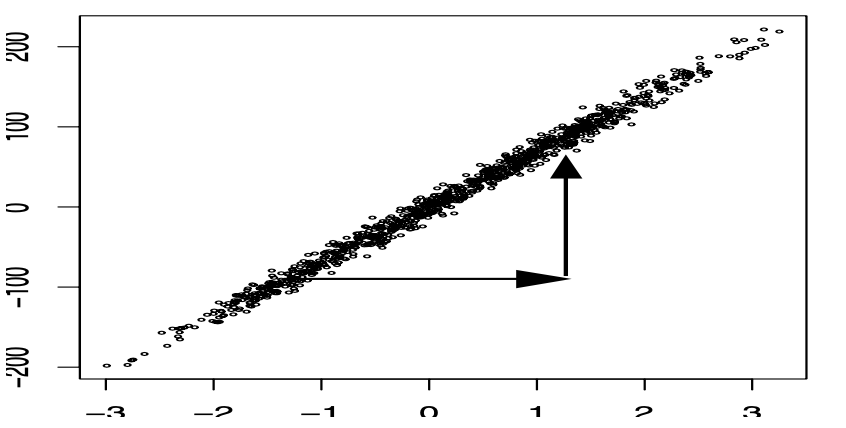
\includegraphics[width = \textwidth]{Figures/RueHeldBookFig.png}
	\caption[Correlation structure in between parameters and hyper-parameters]{The figure taken from~\cite[Figure 4.1 (b)]{rue2005gaussian} shows samples from the chain of $\mu$ (x-axis) and $\bm{1}^T \bm{Q} \bm{x}^{(k)}$ (y-axis) for over 1000 iterations, based on the hierarchical model in Eq.~\ref{eq:rueMod}, with an autoregressive process encoded in $\bm{Q}$. The algorithm updates $\mu$ and $\bm{x}$ successively from their conditional distributions (see Eq.~\ref{eq:gibbsMu} and Eq.~\ref{eq:gibbsx}). The plot displays $(\mu^{(k)}, \bm{1}^T \bm{Q} \bm{x}^{(k)})$, with $\mu^{(k)}$ on the horizontal axis and $\bm{1}^T \bm{Q} \bm{x}^{(k)}$ on the vertical axis. The slow mixing and convergence of $\mu$ result from its strong dependence on $\bm{1}^T \bm{Q} \bm{x}^{(k)}$, while the sampler permits only axis-aligned (horizontal and vertical) and does not allow diagonal moves, as illustrated by the arrows.}
	\label{fig:RueHeld}
\end{figure}

A solution to the slow mixing problem is to update $(\mu, \bm{x})$ jointly.
Since $\mu$ is one-dimensional, effectively only the marginal density of $\mu$ is needed.
\begin{align}
	\mu^{\star}  &\sim q (\mu^{\star}|	\mu^{(k-1)} ) \\
	\bm{x}^{(k)} | \mu^{\star} &\sim \mathcal{N} (	\mu^{\star}\bm{1}, \bm{Q}^{-1}) 
\end{align}
With a simple MCMC algorithm targeting $ \mu$, one can explore the sample space efficiently and only draw a corresponding sample for $\bm{x}$ from its full conditional once, for instance, the proposal $\mu^{\star}$ has been accepted.

\section{Monte-Carlo Error and Integrated Autocorrelation Time}
\label{ap:IATC}
To assess the error $(\sigma^{(i)})^2$ of a samples-based estimate 
\begin{align}
	\bm{\mu}^{(i)} \coloneqq	\text{E}_{\bm{x}|\bm{y}} [h(\bm{x})] = \frac{1}{N} \sum_{k=1}^{N} h(\bm{x}^{(k)}),
\end{align} 
from the chain $\mathcal{M}^{(i)} = \{\bm{x}^{(1)}, \dots,\bm{x}^{(k)},\dots, \bm{x}^{(s)},\dots, \bm{x}^{(N)}\} \sim \pi(\bm{x}|\bm{y})$, we ignore systematic error due to initialisation bias (burn-in period), but we have to take into account that samples produced by any system or algorithm are correlated.
To derive the IACT, we follow Ulli Wolff's lecture notes \cite{wolff2002LecNot} (or alternatively \cite{wolff2004monte}).

In general, the error of a Monte-Carlo estimate is:
\begin{align}
	(\sigma^{(i)})^2 = \text{var}(\bm{\mu}^{(i)}) =  \text{var}(\text{E}_{\bm{x}|\bm{y}} [h(\bm{x})]) = \Bigg( \frac{1}{N} \sum_{k=1}^{N} h(\bm{x}^{(k)}) - \bm{\mu}^{(i)} \Bigg)^2 \, .
\end{align}
Expanding this summation, we see that
\begin{align}
	(\sigma^{(i)})^2 = \frac{1}{N^2} \sum_{k,s=1}^{N} \Gamma(k-s)
\end{align}
with the autocorrelation coefficient $\Gamma(k-s) =  \big( h(\bm{x}^{(k)}) - \bm{\mu}^{(i)} \big) \big(h(\bm{x}^{(s)}) - \bm{\mu}^{(i)} \big)$.
Next we rewrite
\begin{align}
	\sum_{k,s=1}^{N} \Gamma(k-s) = \text{var}(h(\bm{x}))  \sum_{k,s=1}^{N} \frac{\Gamma(k-s)}{\Gamma(0)} =  \text{var}(h(\bm{x})) \sum_{k,s=1}^{N}\rho(k-s)\, ,
\end{align}
with the normalised autocorrelation coefficient $\rho(k-s) =  \Gamma(k-s)/ \Gamma(0)$ at lag $k-s$ and $\Gamma(0) = \text{var}(h(\bm{x}) )$ for $k=s$.
Typically $\Gamma(t)$ decays exponentially so that, for $N\gg \tau$, $\Gamma(t) \overset{t \rightarrow \infty }{ \propto} \exp\{ - |t| / \tau \}  $ and we can approximate
\begin{align}
	\sum_{k,s=1}^{N}\rho(k-s)  = N \sum_{t = -(N-1) }^{N-1} \Bigg(1- \frac{t}{N} \Bigg) \rho(t)  \approx N  \sum_{t = - \infty }^{\infty} \rho(t) \, ,
\end{align}
see \cite[p. 137]{Sokal1997}.
If $\tau \gg 1$
\begin{align}
	\sum_{t = - \infty }^{\infty} \rho(t) =  1 + 2 \sum_{t = 1}^{\infty} \big(e^{-1/ \tau}\big)^t =  1 + 2 \frac{e^{-1/ \tau} }{1 - e^{-1/ \tau}} \approx  1 + 2 \frac{1 -1/ \tau }{1/ \tau} =  2 \tau -1 \approx 2 \tau_{int}\, ,
\end{align}
so that $\tau_{\text{int}} \approx \tau$.
Here we use the geometric power series $\sum^{\infty}_{n=0} x^n= 1/ (1-x)$ and the Taylor series $ e^x \approx 1+x$ for small $x$.
In practise, the estimate for the Monte-Carlo error is:
\begin{align}
	(\sigma^{(i)})^2   \approx \frac{\text{var}(h(\bm{x}) )}{N} \sum_{t = - \infty }^{\infty} \rho(t)
	\approx \frac{\text{var}(h(\bm{x}) )}{N} \Bigg( \underbrace{  1 + 2 \sum_{t = 1}^{W} \rho(t)  }_{ \coloneqq 	2\tau_{\text{int}} }\Bigg) = \text{var}(h(\bm{x})) \frac{ 2 \tau_{\text{int}} }{N}\, ,
\end{align}
where $W$ is the summation window and we define the IACT as in \cite[pp. 103-105]{wolff2002LecNot}.
The IACT provides a good estimate of how many steps the sampling algorithm needs to take to produce one independent sample.
More specifically, the effective sample size $\frac{ 2 \tau_{\text{int}} }{N}$ gives an estimate of how efficient a sampler is.

%\section{Measure Theory}
%\label{ch:Mesure}
%Assume that the triple $(\Omega, \mathcal{F}, \mathbb{P})$ defines a probability space, where $\Omega$ denotes the complete sample space, $\mathcal{F}$ is a $\sigma$-algebra consisting of a collection of countable subsets $\{A_n\}_{n \in \mathbb{N}}$ with $A_n \subseteq \Omega$, and $\mathbb{P}$ is a probability measure on $\mathcal{F}$. The formal conditions for $\mathbb{P}$ to be a probability measure, and for $\mathcal{F}$ to be a $\sigma$-algebra over $\Omega$, are given in Appendix~\ref{ch:Mesure}.
%We denote
%\begin{align}
%	\mathbb{P}(A) = \int_A \diff  \mathbb{P}
%\end{align}
%as the probability of an event $A \in \mathcal{F}$.
%By applying the Radon-Nikodym theorem~\cite{kopp2004measintprob}, we can change variables
%\begin{align}
%	\mathbb{P}(A) = \int_A \frac{\diff \mathbb{P}}{\diff \bm{x}} \, \diff \bm{x} = \int_A \pi(\bm{x}) \, \diff \bm{x},
%\end{align}
%where $\mathrm{d}\bm{x}$ is a reference measure on the same probability space, commonly referred to as the Lebesgue measure. 
%The Radon-Nikodym derivative $\frac{\mathrm{d} \mathbb{P}}{\mathrm{d}\bm{x}}$ of $\mathbb{P}$ with respect to $\bm{x}$ is often interpreted as the probability density function (PDF) $\pi(\bm{x})$. Thus, we say that $\mathbb{P}$ has a density $\pi(\bm{x})$ with respect to $\bm{x}$~\cite[Chapter 10]{simonnet1996measprob}.
%
%Now, let $X: \Omega \longrightarrow \mathbb{R}^d$ be a $d$-dimensional random variable mapping from the probability space $(\Omega, \mathcal{F}, \mathbb{P})$ to the measurable space $(\mathbb{R}^d, \mathcal{X})$, where $\mathcal{X}$ is a collection of subsets in $\mathbb{R}^d$ \cite{VesaInvLect}.
%Then the associated PDF $\pi(\bm{x})$ is a joint density of $X$, induced by the probability measure on $\Omega$~\cite{VesaInvLect, kopp2004measintprob}.
%
%
%Recall the probability space $(\Omega, \mathcal{F}, \mathbb{P})$, where $\Omega$ denotes the sample space, and $\mathcal{F}$ is a collection of countable subsets $\{ A_n \}_{n \in \mathbb{N}}$ of $\Omega$. Each $A_n \subseteq \Omega$ is called an event, and a map $\mathbb{P} : \mathcal{F} \rightarrow \mathbb{R}$ is referred to as a measure.
%In the following, we describe the conditions required for $\mathcal{F}$ to be a $\sigma$-algebra, and for $\mathbb{P}$ to qualify as a probability measure.
%We refer to \cite{lawler2016notes} \cite{kopp2004measintprob} for further reading.
%
%\subsection{Probability Measure}
%For a probability measure, we require:
%\begin{itemize}
%	\item $\mathbb{P}(\Omega) = 1$ and $\mathbb{P}(\emptyset) = 0$
%	\item $\mathbb{P}(A) \in [0,1]$
%	\item $\mathbb{P}(\bigcup_{j \in \mathbb{N}} A_j )= \sum_{j \in \mathbb{N}}  \mathbb{P}(A_j)$ if we have pairwise disjoint sets or $A_i \cap A_j = \emptyset$ for $i \neq j $
%\end{itemize}
%In other words, the probability assigned to the entire sample space must be equal to one, $\mathbb{P}(\Omega) = 1$, and the probability of the empty set must be zero, $\mathbb{P}(\emptyset) = 0$. For any subset $A \subseteq \Omega$, the probability $\mathbb{P}(A)$ must lie between zero and one, i.e., $\mathbb{P}(A) \in [0,1]$.
%If e.g. two subsets $A$ and $B$ are disjoint (i.e., $A \cap B = \emptyset$), then the probability of their union satisfies $\mathbb{P}(A \cup B) = \mathbb{P}(A) + \mathbb{P}(B)$.
%This property must also hold for a countable sequence of disjoint sets $\{A_j\}_{j \in \mathbb{N}}$, such that $\mathbb{P}\left( \bigcup_{j \in \mathbb{N}} A_j \right) = \sum_{j \in \mathbb{N}} \mathbb{P}(A_j)$.
%
%\subsection{$\sigma$-Algebra}
%A collections of subsets $\mathcal{F}$ is called $\sigma$-algebra if:
%\begin{itemize}
%	\item $\emptyset, \Omega \in \mathcal{F} $,
%	\item if $A \in \mathcal{F} $ then $A^C \coloneqq A / \Omega \in \mathcal{F}$
%	\item if $A_1 , A_2, \dots  \in \mathcal{F} $ then $ \bigcup_{j \in \mathbb{N}}  A_j \in  \mathcal{F}$
%\end{itemize}
%In other words, the empty set $\emptyset$ and the entire sample space $\Omega$ must always be elements of $\mathcal{F}$. If a set $A \in \mathcal{F}$, then its complement $A^C = \Omega \setminus A$ must also be in $\mathcal{F}$. 
%If, in terms of a probability measure, we are able to assign a probability $\mathbb{P}(A)$ to an event $A$, we must also be able to assign a probability to the event “not $A$”, i.e., $\mathbb{P}(A^C)$.
%Finally, if a countable collection of sets $A_1, A_2, \dots \in \mathcal{F}$, then their union $\bigcup_{j \in \mathbb{N}} A_j$ must also be in $\mathcal{F}$. These three properties define the requirements for $\mathcal{F}$ to be a $\sigma$-algebra.
\clearpage
\section{Python Code}
%\the\baselineskip

\begin{lstlisting}[language=Python, columns=flexible, caption={Python code to calculate Backward marginals, as in Prop. \ref{prob:backMarg} and \cite{cui2022deep}.}, escapeinside={"}{"}]
def MargBack(TTCore, univarGrid):
	''' Backward marginalisation (see "Prop. \ref{prob:backMarg}") as in SIRT from Cui et al. "\cite{cui2022deep}" '''
	
	dim = len(univarGrid)
	B = dim * [None]  # coeffTensor
	B[-1] = TTCore[-1]
	R = [None] * dim
	C = [None] * dim
	
	for k in range(dim - 1, 0, -1):
		r_kmin1, n, r_k = np.shape(TTCore[k])
		# "Eq. \ref{eq:MassMat}, \cite[Eq. 22]{cui2022deep}" !! we set Lebesgue Measure to const = one
		M = np.identity(n) * (univarGrid[k][-1] - univarGrid[k][0])  # Mass matrix
		L = scy.linalg.cholesky(M)
		
		# construct Tensor C  "Eq. \ref{eq:constrCBack}, \cite[Eq. 27]{cui2022deep}"
		C[k] = np.zeros((r_kmin1, n, r_k))
		for alpha in range(0, r_kmin1):
			for l in range(0, r_k):
				C[k][alpha, :, l] = B[k][alpha, :, l] @ L[:, :]
		
		# unfold along first coordinate and compute thin QR decomposition of C^T
		#  "Eq. \ref{eq:thinQRBack}, \cite[Eq. 28]{cui2022deep}"
		Q, R[k] = np.linalg.qr(C[k].reshape((r_kmin1, n * r_k), order='C').transpose(), mode='reduced')
		
		# compute next coefficient tensor "Eq. \ref{eq:nextCoeffTBack}, \cite[Eq. 29]{cui2022deep}"
		r_kmin2, n, r_kmin1 = np.shape(TTCore[k - 1])
		B[k - 1] = np.zeros(np.shape(TTCore[k - 1]))
		for alpha_2 in range(0, r_kmin2):
			for l_1 in range(0, r_kmin1):
				B[k - 1][alpha_2, :, l_1] = TTCore[k - 1][alpha_2, :, :] @ R[k][l_1, :]

return B

\end{lstlisting}
\clearpage
\begin{lstlisting}[language=Python, columns=flexible, caption={Python code to calculate forward marginals, as in Prop. \ref{prob:ForMarg}.}, escapeinside={"}{"}]
	def MargForw(TTCore, univarGrid):
	''' Forward marginalisation (see "Prop. \ref{prob:ForMarg}") 
		similar to backward marginalsiation as in  Cui et al. "\cite{cui2022deep}" '''
	
	# compute pre marginal coefficients sarting at dim = 1, k = 0
	BPre = dim * [None]  # coeffTensor
	LebLam = 1  # !! Lebesgue Measure
	BPre[0] = TTCore[0]
	RPre = [None] * dim
	CPre = [None] * dim
	
	for k in range(0, dim-1):
		r_kmin1, n, r_k = np.shape(TTCore[k])
		#  "Eq. \ref{eq:MassMat}, \cite[Eq. 22]{cui2022deep}" !! we set Lebesgue Measure to const = one
		M = np.identity(n) * (univarGrid[k][-1] - univarGrid[k][0])  # Mass matrix
		L = scy.linalg.cholesky(M)
		
		# construct Tensor C  "Eq. \ref{eq:constrCForw}"
		CPre[k] = np.zeros((r_kmin1, n, r_k))
		for alpha in range(0, r_kmin1):
			for l in range(0, r_k):
				CPre[k][alpha, :, l] = BPre[k][alpha, :, l] @ L[:, :]
		
		# unfold along first coordinate and compute thin QR decomposition of C
		# "Eq. \ref{eq:thinQRForw}"
		Q, RPre[k] = np.linalg.qr(CPre[k].reshape((r_kmin1 * n, r_k), order='C'), mode='reduced')
		
		# compute next coefficient tensor  "Eq. \ref{eq:nextCoeffTForw}"
		r_k, n, r_kpls1 = np.shape(TTCore[k + 1])
		BPre[k + 1] = np.zeros(np.shape(TTCore[k + 1]))
		for alpha_1 in range(0, r_kpls1):
			for l_1 in range(0, r_k):
				BPre[k + 1][l_1, :, alpha_1] = RPre[k][l_1,:] 
					"\phantom{$BPre[k + 1][l_1, :, alpha_1] = RPre[k][l_1,:] $}"@ TTCore[k + 1][:, :, alpha_1]
		
	return BPre
	
\end{lstlisting}


\clearpage
\begin{lstlisting}[language=Python,	columns=flexible, caption = {Python code to draw samples via SIRT, as in Alg. Box \ref{alg:SIRT}.}, escapeinside={"}{"}]
def SIRT(seeds, SQTT, univarGrid, BackMarg, absError):
	''' do squared inverse rosenblatt transform (SIRT) as in Cui et al. "\cite{cui2022deep}" '''
	
	dim, numbSampl = seeds.shape
	sampls = np.zeros(seeds.shape) # samples from approximated PDF
	probVal = np.zeros(seeds.shape) # PDF values, for MH-correction step
	Approx = np.zeros(seeds.shape[1]) # TT-Approx., to compare to true function
	
	# Lebesgue measure for quadrature "Eq. \ref{eq:lebesgueWeight}"
	WholeLebLam = np.zeros(dim)
	for k in range(0, dim):
		WholeLebLam[k] = (univarGrid[k][-1] - univarGrid[k][0])
	lamX = np.ones(dim)
	for k in range(1, dim):
		lamX[k - 1] = np.prod(WholeLebLam[k:])
	
	
	gamError = absError / np.prod(WholeLebLam) # error as in "Eq. \ref{eq:gamErr} \cite[Eq. (35)]{cui2022deep}"
	
	# sample from first dimension "\cite[Eq. (30)]{cui2022deep}"
	firstMarg = gamError * lamX[0] + np.sum(BackMarg[0][0, :, :] ** 2, 1)
	# cumulative distribution function, normalised numerically "Eq. \ref{eq:CurrCDF} \cite[Eq. (17)]{cui2022deep}"
	firstCDF = np.cumsum(firstMarg / np.sum(firstMarg))
	# draw samples as 'inverse transform'
	sampls[0] = np.interp(seeds[0], firstCDF, univarGrid[0])
	probVal[0] = np.interp(sampls[0], univarGrid[0], firstMarg / np.sum(firstMarg))
	
	# sample from other dimensions
	for n in range(0, numbSampl):
		# piecew. poly. interpol in first dimension "Eq. \ref{eq:LinPol} \cite{dolgov2020approximation}"
		CurrApprCore = LinInterPolTT(SQTT[0], univarGrid[0], sampls[0][n])
		for d in range(1, dim):
			# marginal function, conditioned on previous samples
			rank_min, gridSize, rank_pls = BackMarg[d].shape
			MargDep = np.zeros((BackMarg[d].shape))
			for r in range(0, rank_min):
				# condition on previous samples
				MargDep[r, :, :] = CurrApprCore[0, r] * BackMarg[d][r, :, :]
			
			currMarg = gamError * lamX[d] + np.sum(np.sum(np.copy(MargDep), axis=0)** 2,
				axis=1) # "Eq.~\ref{eq:CurrMarg}~\cite[Eq. (31)]{cui2022deep}"
			
			currCDF = np.cumsum(currMarg / np.sum(currMarg)) # "Eq. \ref{eq:CurrCDF} \cite[Eq. (17)]{cui2022deep}"
			
			# draw sample as 'inverse transform'
			sampls[d][n] = np.interp(seeds[d][n], currCDF, univarGrid[d])
			probVal[d][n] = np.interp(sampls[d][n], univarGrid[d],  
				currMarg / np.sum(currMarg))
			# piecew. poly. interpol., "Eq. \ref{eq:LinPol}~\cite{dolgov2020approximation}", cond. on sampl. for next PDF
			CurrApprCore = np.copy(CurrApprCore) @ LinInterPolTT(SQTT[d], univarGrid[d], 
				sampls[d][n]) 
	
	Approx[n] = gamError + CurrApprCore ** 2
	
	return sampls, probVal, Approx
\end{lstlisting}
\clearpage



